% !TEX root = ../../buch.tex
% einleitung.tex -- Beispiel-File für die Einleitung
%
% (c) 2020 Prof Dr Andreas Müller, Hochschule Rapperswil
%
\section{Einleitung \label{burgers:section:einleitung}}
\rhead{Einleitung}
	
	Die Gleichung von Burgers,
	\begin{equation}
		  \frac {\partial u}{\partial t}+u{\frac {\partial u}{\partial x}}=\nu {\frac {\partial ^{2}u}{\partial x^{2}}},
		  \label{burgers:eq_burgers}
	\end{equation}
	ist eine nichtlineare partielle Differentialgleichung.
	Sie beschreibt die Amplitude $u$ in Funktion der Zeit und dem Raum.
	In diesem Paper wird die reibungsfreie Burgersgleichung, 
	\begin{equation}
		\frac {\partial u}{\partial t}+u{\frac {\partial u}{\partial x}}=0,
		\label{burgers:eq_invisid_burgers}
	\end{equation}
	betrachtet, wobei der Diffusionsterm $\nu$ auf 0 gesetzt wird.
	
	Als Beispiel kann f\"ur die Startbedingung eine Normalverteilung verwendet werden.
	Die gel\"oste Gleichung kann in \ref{burgers:fig:b1} betrachtet werden.
	
	    \begin{figure}
		\centering
		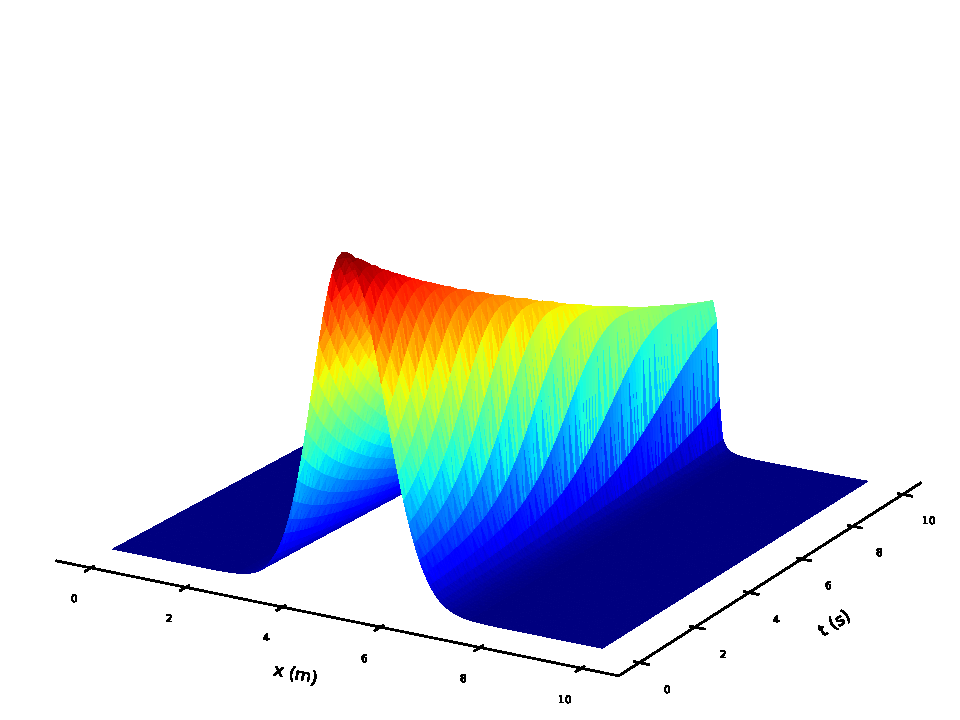
\includegraphics[width=.49\textwidth]{papers/burgers/BurgersEquation/images/Implicit_front.pdf}
		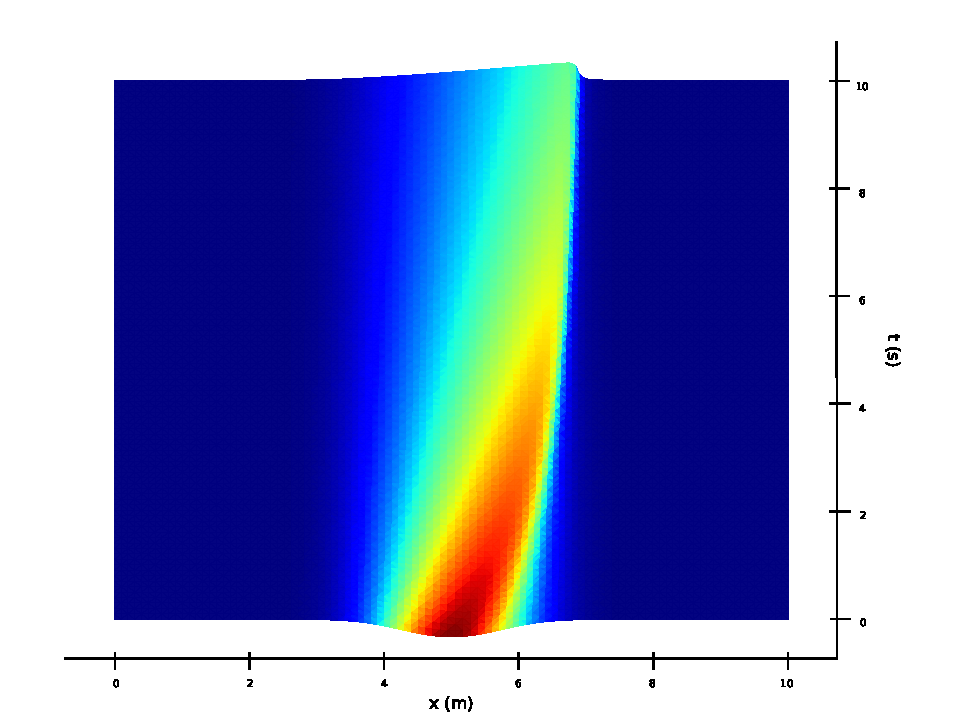
\includegraphics[width=.49\textwidth]{papers/burgers/BurgersEquation/images/Implicit_top.pdf}
		\caption{Gel\"oste Burgersgleichung}
		\label{burgers:fig:b1}
		\end{figure}
	
	
	\subsection{Beziehung zu den Navier Stokes Gleichungen}
		Die Gleichung kann als Vereinfachung von komplexeren Themen verwendet werden.
		Namentlich wird sie gebraucht um die Navier Stokes Gleichungen zu vereinfachen.
		Die Navier Stokes Gleichungen modellieren die Str\"omung von Fluiden.
		Die Gleichung von Burgers kann aus der Navier Stokes Gleichung f\"ur newtonsche inkompressible Fluide hergeleitet werden. \cite{burgers:navier}
		
		
		\begin{equation}
			\rho \left(\frac{\partial u}{\partial t} + u \, \nabla u \right) = -\nabla p + \mu \nabla^2 u + F 	
			\label{burgers:eq_navier}
		\end{equation}
		Wenn der Druck $p$ und die externe Kraft $F$ vernachl\"asigt wird, ergibt sich
		\begin{equation}
			\rho \left(\frac{\partial u}{\partial t} + u \, \nabla u \right) = \mu \nabla^2 u
			 \label{burgers:eq_navier2}
		\end{equation}
		Die Dichte $\rho$ kann mit der Geschwindigkeit des Vektorfeldes $\mu$ zur Konstante $\nu = \frac{\mu}{\rho}$ umgeschrieben werden.
		
		\begin{equation}
			 \frac{\partial u}{\partial t} + u \,\nabla u = \nu \nabla^2 u 
			 \label{burgers:eq_navier3}
		\end{equation}
		
		Wie bereits erw\"ahnt wird die reibungsfreie Gleichung betrachten ($\nu = 0$), weiter werden die kommenden Betrachtungen im Eindimensionalen Raum durchgef\"uhrt.
		Somit kann der Ableitungsoperator $\nabla$ als die Ableitung im Raum $x$ umgeschrieben werden.
		Somit ist man mit den Vereinfachungen der Navier Stokes Gleichungen beendet und bei der urspr\"unglichen Gleichung \eqref{burgers:eq_invisid_burgers} angelangt.
	
	%\subsection{Numerische Wetter Vorhersage}
	%	Lewis Fry Richardson (1881 - 1953) war ein Britischer Mathematiker/Physiker.
		